\section{Projektbeschreibung und Projektziele}
Für den praktischen Teil dieser Arbeit soll anhand der Entwicklung einer Ruby-on-Rails\hyp{}Anwendung die Testgetriebene Entwicklung erprobt und angewendet werden.

Als Ergänzung zu den lokalspezifischen Communitys mit strenger Mitgliederauswahl soll nun ein neues, allgemeines IT-Jobportal entwickelt werden. Der vorraussichtliche Name wird IT-Jobs-Und-Stellen.de\footnote{\url{http://www.it-jobs-und-stellen.de/}} sein.

Ziel soll es sein, den regionalen Organisationen auch eine Alternative zu den Community-Mitgliedschaften anzubieten, um kurzfristigen Personalbedarf zu decken, analog zu den bekannten Online-Stellenbörsen stepstone.de, monster.de und jobscout24\footnote{\url{http://www.stepstone.de} - \url{http://www.monster.de} - \url{http://www.jobscout24.de}}. Parallel zu dieser Arbeit wurden die Anforderungen analysiert und die in Abbildung \ref{fig:usecases} dargestellten Anwendungensfälle bestimmt.


\begin{figure}[htbp]
 \centering
 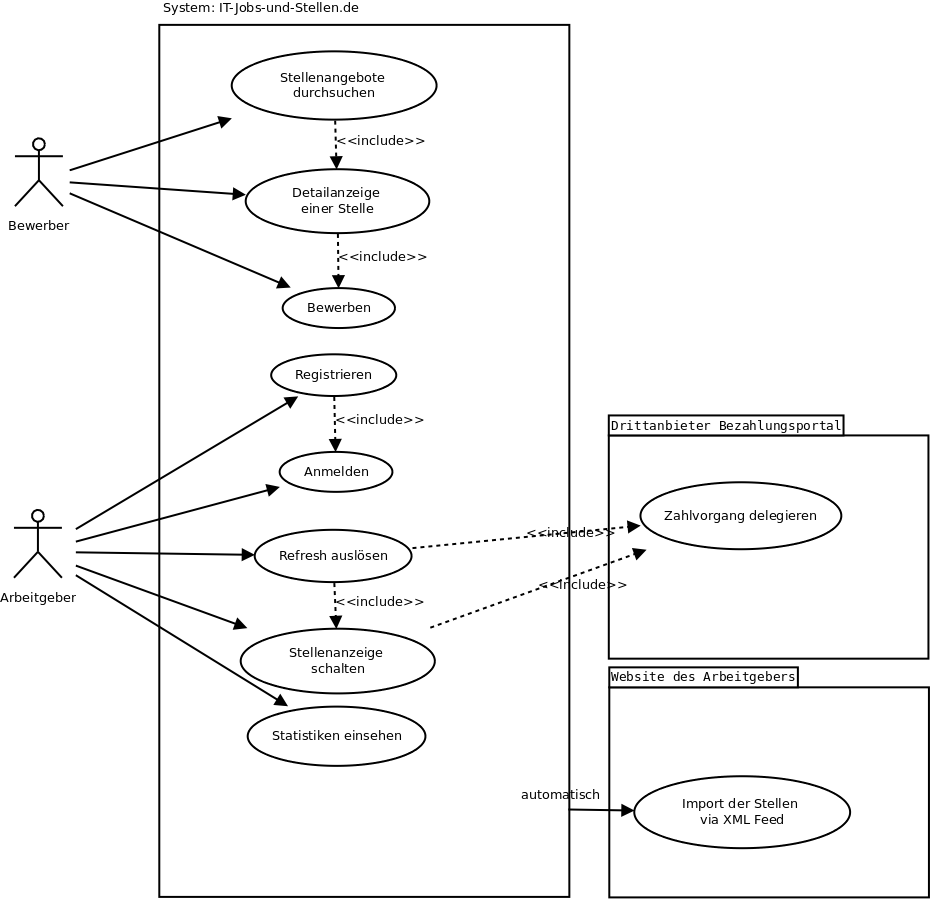
\includegraphics[width=1\textwidth]{./material/usecases.png}
 % usecases.png: 930x899 pixel, 51dpi, 46.50x44.95 cm, bb=
 \caption{Anwendungsfälle}
 \label{fig:usecases}
\end{figure}


\subsection{Anwendungsfälle}
Es gibt zwei verschiedene Nutzertypen. Zum einen, ein \textit{Bewerber}, der das Ziel hat einen Job zu suchen, zu finden und sich darauf zu bewerben. Zum anderen ein Mitarbeiter eines Kundenunternehmenes (\textit{Arbeitgeber}), der Jobs auf der Webseite schalten möchte.
Verbal formuliert sind die Anwendungsfälle die folgenden:
\begin{itemize}
 \item Ein Bewerber kann die Webseite nach sichtbaren Stellenangeboten durchsuchen.
 \item Ein Bewerber kann die Detailanzeige einer Stelle betrachten.
 \item Ein Bewerber kann sich auf eine Stelle über das System bewerben. Dabei kann er auch eine Verbindung zu seinem Facebook- oder LinkedIn-Account herstellen, falls er das möchte, um so automatisch einen Lebenslauf generieren zu lassen und Stammdaten eintragen zu lassen.
 \item Ein Kunde kann sich am Portal registrieren und dann anmelden, und wird so zum \textit{Arbeitgeber}.
 \item Ein Arbeitgeber kann eine Stellenanzeige für ein Vielfaches von 30 Tagen schalten. Damit wird ein Bezahlvorgang über einen Drittanbieterportal (z.B. paypal) ausgelöst und bei Bestätigung die Stelle sichtbar geschaltet. Er kann dazu zwischen 5 verschiedenen Designs wählen, und Logo und Bild hinzufügen.
 \item Ein Arbeitgeber kann eine Stelle verlängern oder kopieren und als Vorlage für ein neues Stellenangebot nutzen.
 \item Ein Arbeitgeber kann eine laufende Stelle erneuern (refresh), und so seine Platzierung verbessern. Dies ist möglich, weil die Aktualität einer Stelle Auswirkungen auf die Platzierung in den Suchergebnissen hat. Ein Refresh kostet Geld und löst somit wieder einen Bezahlvorgang aus.
 \item Ein Arbeitgeber kann Statistiken über seine geschalteten Stellenanzeigen einsehen. Dies beinhaltet die Anzahl der Zugriffe pro Tag, Anzahl der Bewerbungen je Stelle.
 \item Ein Arbeitgeber kann seine Stellen mittels eines XML-Feed-Imports automatisiert einlesen. Dazu bezahlt er einen Pauschalbetrag je Kalenderjahr. Das System liest alle 6h automatisert diesen Feed ein, der durch HTTP erreichbar sein muss, und überträgt gültige Stellenanzeigen in die Datenbank. Nicht mehr in dem Feed enthaltene Stellenanzeigen des Arbeitgebers werden in der Datenbank auf "`unsichtbar"' gesetzt. Das Format ist eine Modifikation von \glossar{RSS} 2.0.
\end{itemize}



\subsection{Nichtfunktionale Anforderungen}
Folgende Rahmenbedingungen und zusätzliche Ziele wurden vereinbart.

\begin{itemize}
 \item Eine hohe C0-\glossar{Testabdeckung} von mindestens 95\% als Grundlage für weitere Arbeiten und für den Prozess der \glossar{TDD}
 \item Eine hohe Erweiterbarkeit, um langfristig auch die bereits vorhandenen Communityportale durch das neue System zu ersetzen, welche gegenwärtig auf dem Framework \textbf{Drupal} 5 (PHP) basieren
 \item Eine moderne Suchfunktion durch einen Suchdaemon, z.B. Sphinx oder Lucene
 \item Softwarestack: Ruby 1.9.2 mit Ruby on Rails 3.1, Javascript\index{Javascript} mit JQuery 1.6
 \item Die Software soll eine möglichst einfache und eingängige Bedienung haben
\end{itemize}

